% Figure 4: (a) subtraction mean, (b) activation maps. Each PNG already holds both
% noOVS | OVS montages, the shared colorbar, the joint title and the white corner labels
% (../matlab/fig4_generate.m); this only stacks them and adds the panel letters.
% Build (from latex_fig/): pdflatex -output-directory=../figures_assembled fig4.tex
\documentclass[tikz,border=2pt]{standalone}
\usepackage{graphicx}
\usepackage{helvet}
\renewcommand{\familydefault}{\sfdefault}
\usetikzlibrary{arrows.meta,calc}

\def\W{17cm}     % width of each panel
\def\gy{0.3cm}   % gap between panels

\begin{document}
\begin{tikzpicture}
  \node[anchor=north west, inner sep=0] (a)
    {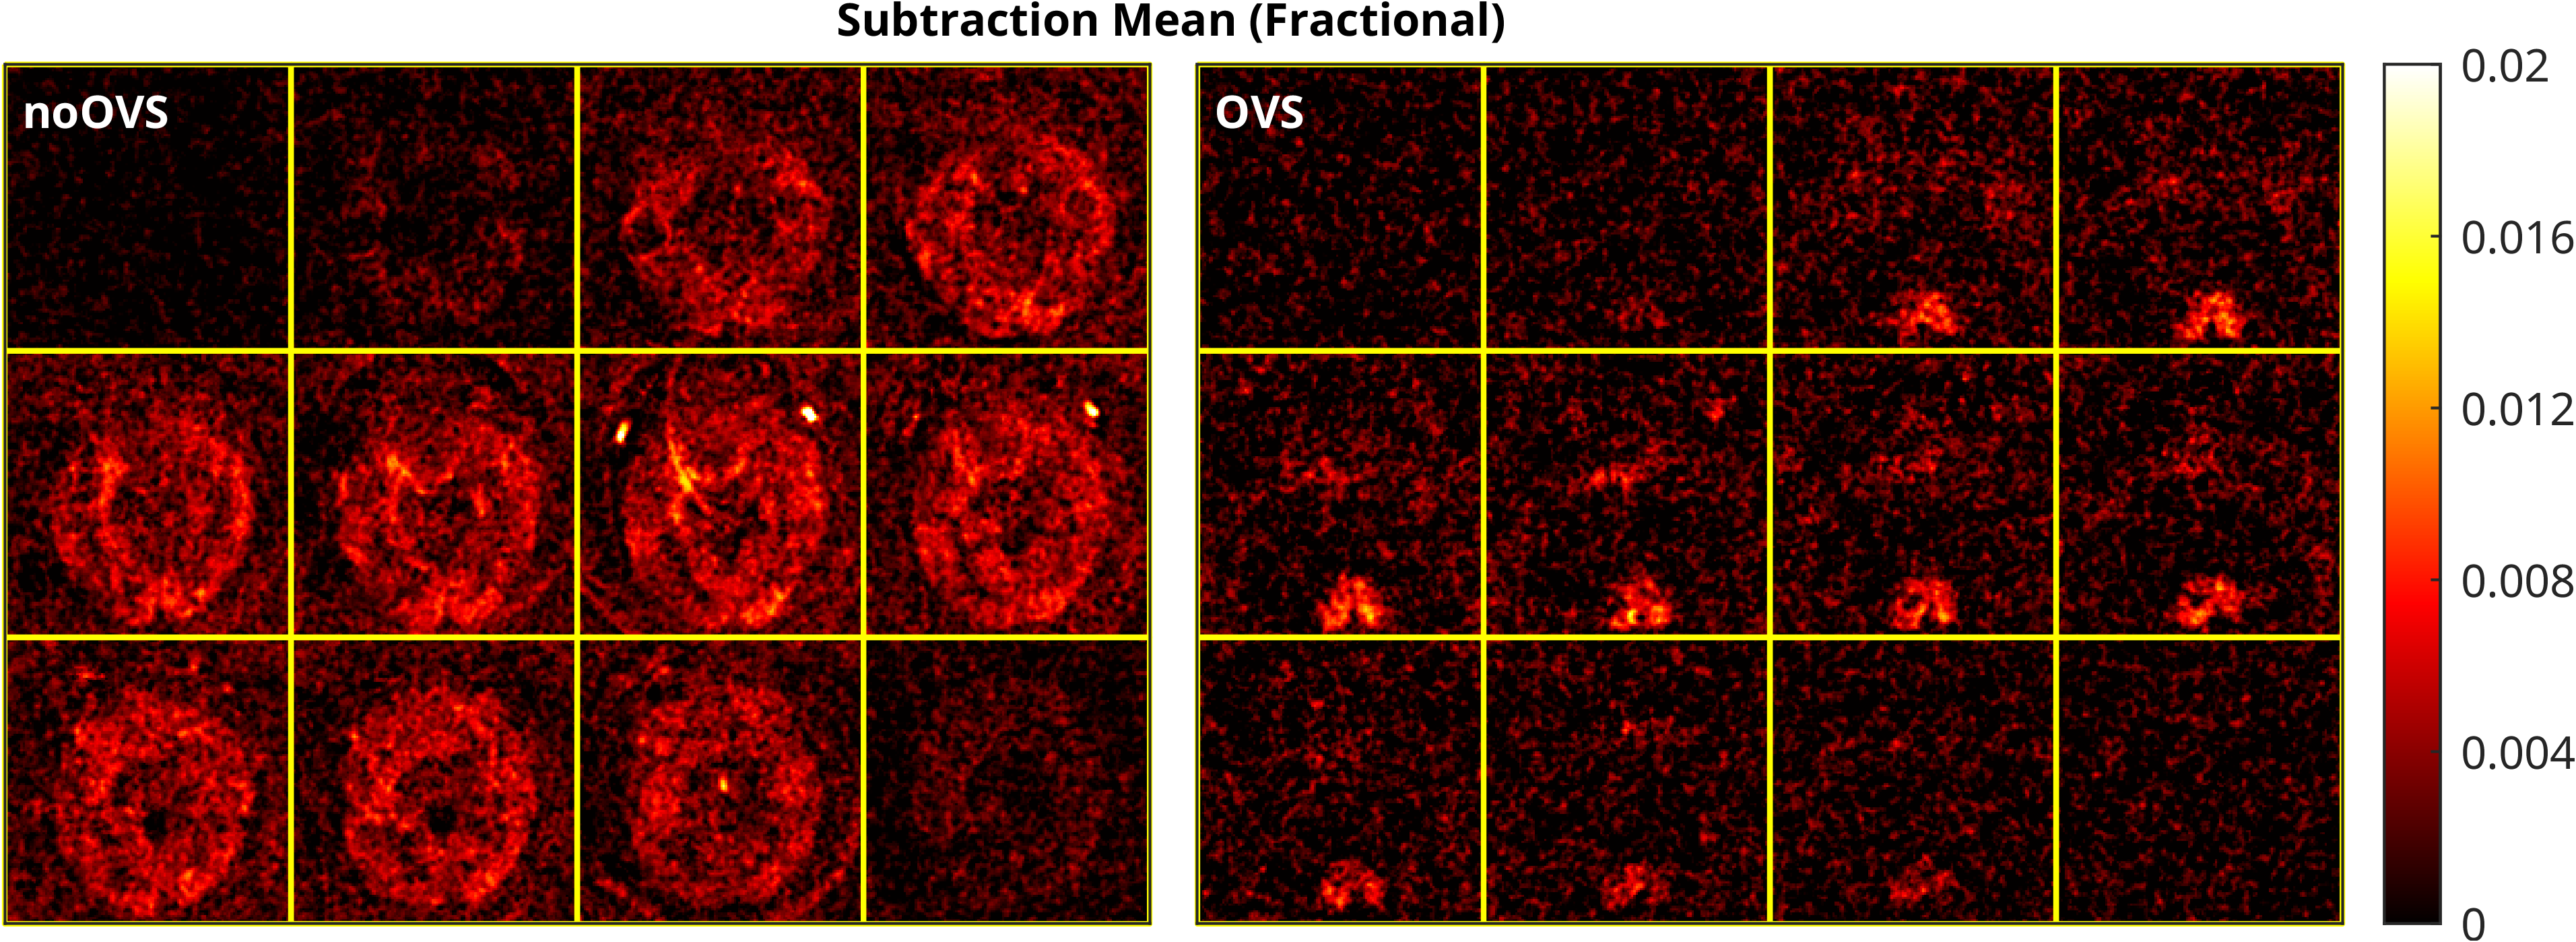
\includegraphics[width=\W]{../figures/fig4_subtraction_mean.png}};
  \node[anchor=north west, inner sep=0] (b) at ([yshift=-\gy]a.south west)
    {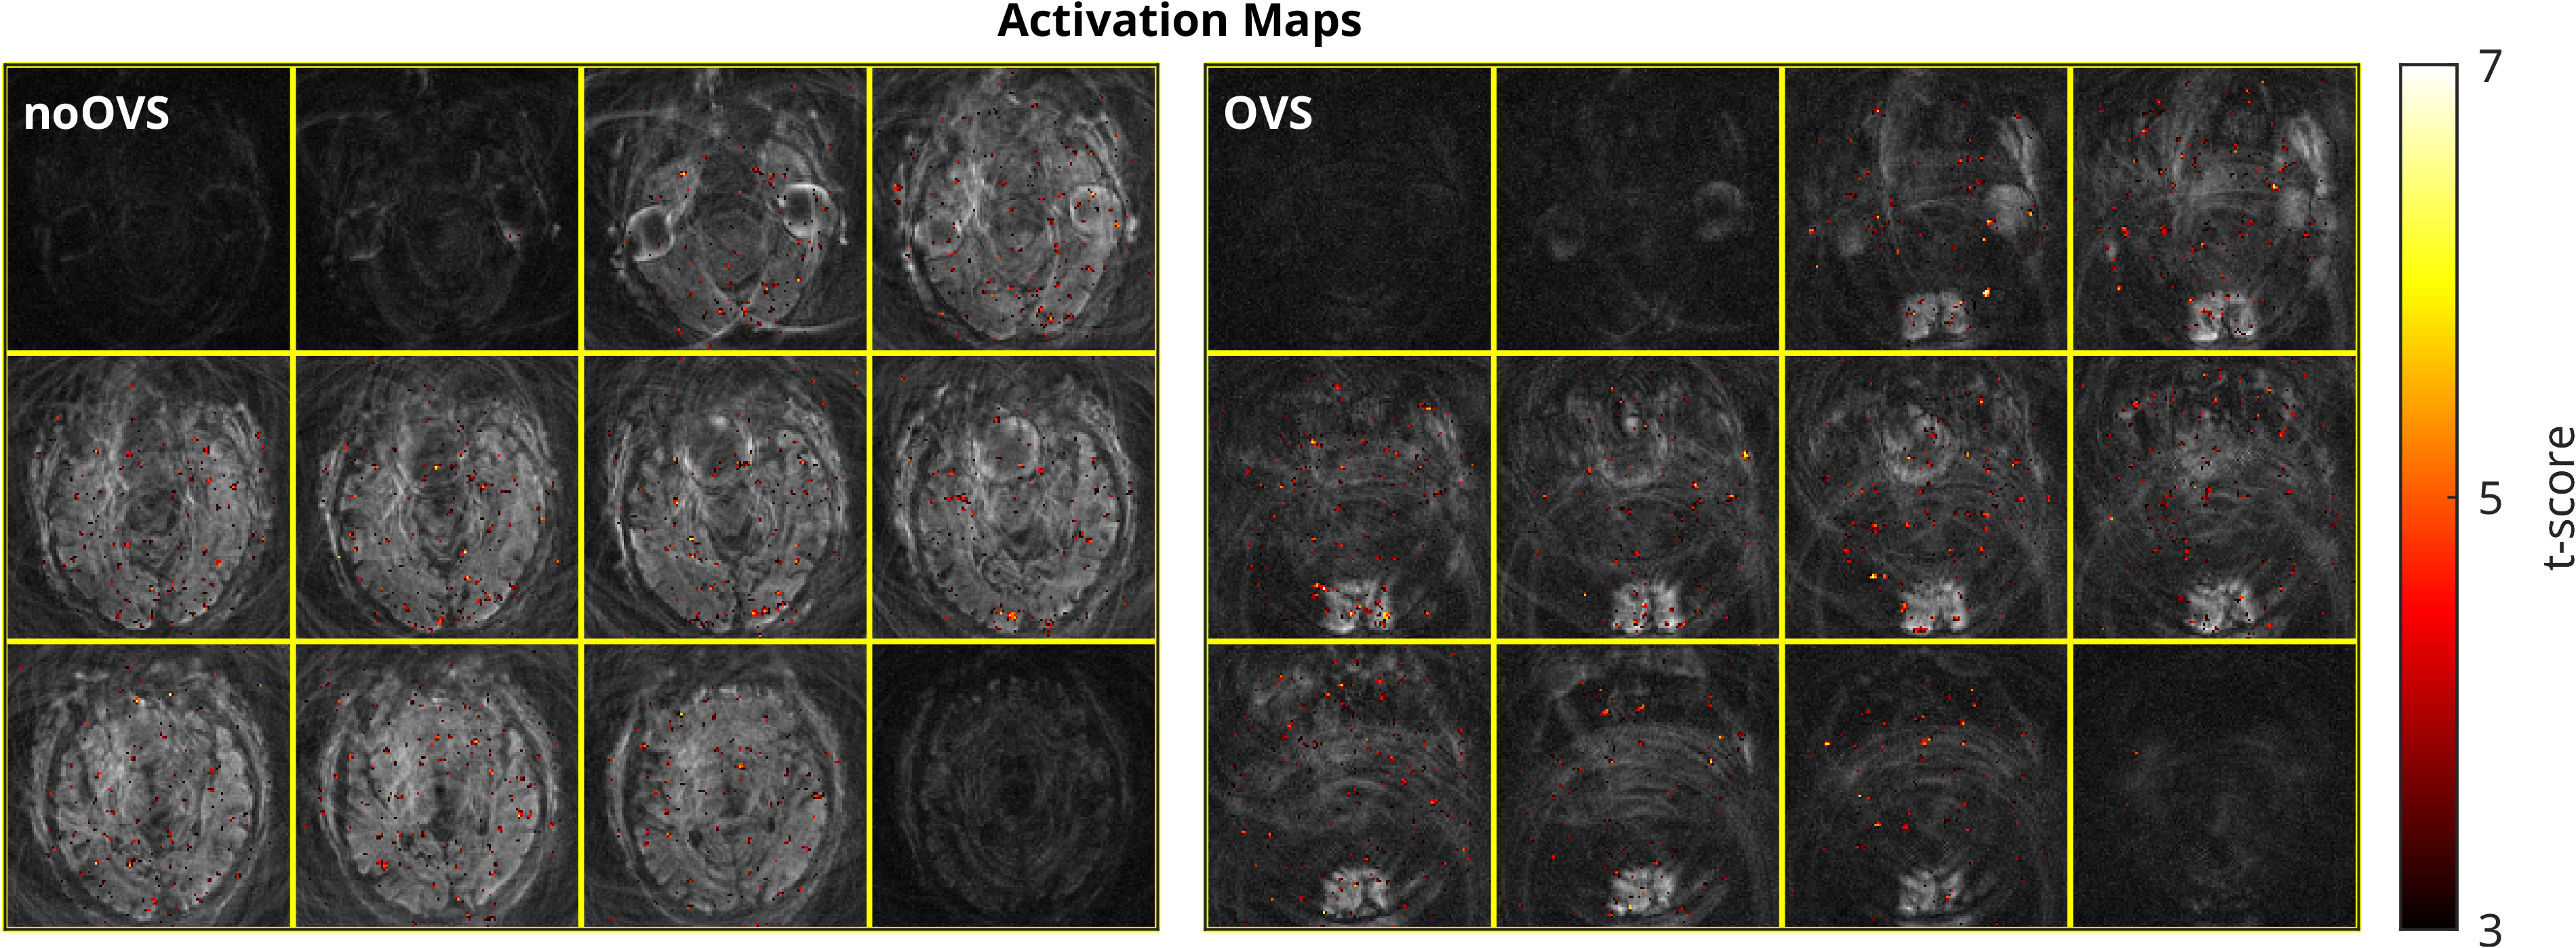
\includegraphics[width=\W]{../figures/fig4_overlay.png}};
  % (b) arrows at the occipital ROI of row 2, column 1, same spot in both montages:
  % OVS shows a cluster there that noOVS lacks. Pixel coords on fig4_overlay.png
  % (3799 x 1398): tile origins (10,524) noOVS and (1781,524) OVS, tile 418 px;
  % arrow from tile (345,305) to (255,380), coming in from the upper right: tip of the right-hemisphere occipital lobe
  % normalized image coordinates of (b): (0,0) bottom-left, (1,1) top-right
  \begin{scope}[shift={(b.south west)}, x={($(b.south east)-(b.south west)$)},
                y={($(b.north west)-(b.south west)$)}]
    \foreach \xo in {10, 1781}
      \draw[-{Stealth[length=2.2mm]}, cyan, line width=1.2pt]
        ({(\xo+345)/3799},{1-829/1398}) -- ({(\xo+255)/3799},{1-904/1398});
  \end{scope}
  \foreach \n in {a,b}
    \node[anchor=north west, font=\bfseries, inner sep=0] at (\n.north west) {(\n)};
\end{tikzpicture}
\end{document}
